\documentclass[DM,toc]{lsstdoc}
\usepackage{booktabs}

\title[Early Qserv Tests]{Early (pre-2013) Qserv Tests}
\author{Jacek~Becla, K-T Lim, Daniel Wang}
\date{2013-08-02}
\setDocRef{DMTR-21}

\setDocAbstract{%
This test report contains Qserv large-scale tests that were performed during the research and development phase.
The format is non-standard as it combines many tests of different aspects of Qserv performed over a number of years.
All the tests were performed in early 2013 or earlier.
Many of these tests were originally documented on the LSST Trac, and versions of \citeds{LDM-135} from 2013 and earlier.
}

\begin{document}
\maketitle

\section{Large-scale Testing}\label{large-scale-testing}

\subsection{Introduction}\label{introduction-1}

\subsubsection{Ideal environment}\label{ideal-environment}

Based on the detailed spreadsheet analysis, we expect the ultimate LSST
production system will be composed of few hundred database servers
\citedsp{LDM-144}, so a realistic test should include a cluster of at
least 100 nodes.

Total database size of a single data release will vary from
\textasciitilde{}1.3\,PB (DR1) to \textasciitilde{}15\,PB
(DR11).\footnote{These numbers are for single copy, data and indices,
  compressed when appropriate.} Realistic testing requires at least
\textasciitilde{}20-30\,TB of storage (across all nodes).

Note that \emph{a lot} of highly focused tests which are extremely
useful to fine tune different aspects of the system can be done on a
very small, 2-3 cluster, or even on a single machine. An example of that
can be measuring the effect of table size on the performance of
near-neighbor join: this type of join will be done per sub-partition,
and sub-partitions will be small (few K rows), thus almost all tests
involving a single sub-partition can be done on a single machine with
very little disk storage.

A significant amount of testing should be done where the dataset size
exceeds the system memory size by an order of magnitude. This testing is
important to reveal system performance in the presence of disk
performance characteristics.

It is essential to have at least two different types of catalogs: Object
and Source. Of course this data needs to be correlated, that is, the
objects should corresponds to the sources. Having these 2 tables will
allow us to measure speed of joins. It is not necessary to have other
types of source-like tables (\DIASource, \ForcedSource) -- the tests done
with \Source should be a good approximation.

The most important characteristic of the test data is its spatial
distribution. The data should reflect realistic densities: presence of
very crowded or very sparse regions have influence on how data is
partitioned and on performance of certain queries (e.g., speed of near
neighbor inside one partition). Other than realistic spatial
distribution, we need several fields to be valid (e.g., magnitudes) in
order to try some queries with predicates.

These tests are not only used to prove our system is capable of meeting
the requirements, but also as a mean to stress the system and uncover
potential problems and bottlenecks. In practice, whoever runs these
tests should well understand the internals of the scalable architecture
system and turning MySQL.

\subsubsection{Schedule of testing}\label{schedule-of-testing}

\begin{itemize}
\item
  Selecting the base technology -- Q2 2009
\item
  Determining the architecture -- Q3 2009
\item
  Pre-alpha tests focused on parallel distributed query execution
  engine, tests at small scale (\textasciitilde{}20 nodes) -- Q4 2009
\item
  Most major features in (except shared scan, user tables), performance
  tests on mid-size cluster (\textasciitilde{}100 nodes) -- Q4 2010
\item
  Scalability and performance improvements and tests on a large cluster
  (150-250 nodes) -- Q4 2011
\item
  Large scale tests, performance tests on a large cluster (250-300
  nodes) -- Q2 2013
\item
  Shared scans -- Q3 2013
\item
  Fault tolerance -- Q4 2013
\end{itemize}

\subsubsection{Current status of tests}\label{current-status-of-tests}

We have run several large scale tests

\begin{enumerate}
\def\labelenumi{\arabic{enumi}.}
\item
  (10/2009) A test with the ``pre-alpha'' version of our software
  written on top of MySQL, using the \emph{Tuson} cluster at LLNL (160
  nodes, each node: two Intel Xeon 2.4 GHz GPUs with 4 GB RAM and 1
  local hard disk of 80 Gbs)
\item
  (2010) several 100-node tests run at SLAC \citep{slac-test}. These tests helped
  us uncover many bottlenecks and prompted rewriting parts of our
  software, as well as implementing several missing features in
  XRootD.
\item
  (4/2011) A 30 TB test on 150-node SLAC cluster using Qserv in
  40/100/150 node configurations, using 2 billion row Object and 32
  billion row Source tables, total of 30 TB data set.
\item
  (12/2012) A 100-terabyte test on JHU's \emph{Datascope} 20-node
  cluster. Due to high instability of the cluster this test turned into
  testing resilience to faults of Qserv and the associated
  administrative tools.
\item
  (05/2013) A 10,000-chunk test on a 120-node SLAC cluster to reproduce
  and understand subtle issues with concurrency at scale.
\item
  (07/2013) A test on 300-node IN2P3 cluster to re-test scalability,
  performance, concurrency, and uncover unexpected issues and
  bottlenecks.
\item
  (08/2013) A demonstration of shared scans.
\end{enumerate}

The tests 3-5 listed above are described in further details below, with test 6 documented in \citeds{DMTR-12}.

\subsection{150-node Scalability Test}\label{node-scalability-test}

\subsubsection{Hardware}\label{hardware}

We configured a cluster of 150 nodes interconnected via gigabit
Ethernet. Each node had 2 quad-core Intel Xeon X5355 processors with
16GB memory and one 500GB 7200RPM SATA disk. Tests were conducted with
Qserv SVN r21589, MySQL 5.1.45 and XRootD
3.0.2 with Qserv patches.

\subsubsection{Data}\label{data}

We tested using a dataset synthesized by spatially replicating the
dataset from the LSST data challenge (``PT1.1''). We used two tables:
Object and Source.\footnote{The schema may be browsed online at
  \url{http://lsst1.ncsa.uiuc.edu/schema/index.php?sVer=PT1_1}} These
two tables are among the largest expected in LSST. Of these two, the
Object table is expected to be the most frequently used. The Source
table will have 50-200X the rows of the Object table, and its use is
primarily confined to time series analyses that generally involve joins
with the Object table.

The PT1.1 dataset covers a spherical patch with right-ascension between
358˚ and 5˚ and declination between -7˚ and 7˚. This patch was treated
as a spherical rectangle and replicated over the sky by transforming
duplicate rows' RA and declination columns, taking care to maintain
spatial distance and density by a non-linear transformation of
right-ascension as a function of declination. This resulted in an Object
table of 1.7 billion rows (2TB) and a Source table of 55 billion rows
(30 TB).\footnote{Source for the duplicator is available at
  \url{https://github.com/lsst/qserv/blob/master/admin/python/lsst/qserv/admin/dataDuplicator.py}}
The Source table included only data between -54˚ and +54˚ in
declination. The polar portions were clipped due to limited disk space
on the test cluster. Partitioning was set for 85 stripes each with 12
sub-stripes giving a $\phi$ height of \textasciitilde{}2.11˚ for stripes and
0.176˚ for sub-stripes. Each chunk thus spanned an area of approximately
4.5\,deg\textsuperscript{2}, and each sub-chunk,
0.031\,deg\textsuperscript{2}. This yielded 8,983 chunks. Overlap was set
to 0.01667˚ (1 arc-minute).

\subsubsection{Queries}\label{queries}

The current Qserv development focus is on features for scalability. We
have chosen a set of test queries that demonstrate performance for both
cheap queries (interactive latency), and expensive queries (hour, day
latency). Runs of low volume queries ranged from 15 to 20 queries, while
runs of high volume queries and super high volume queries consisted of
only a few or even one query due to their expense. All reported query
times are according to the command-line MySQL client (\emph{MySQL}).

\paragraph{Low-volume 1 -- object
retrieval}\label{low-volume-1-object-retrieval}

\begin{lstlisting}[language=SQL]
SELECT * FROM Object WHERE objectId = <objId>
\end{lstlisting}

In \figref{fig:150-node-low-vol-object-retrieval} we can see that performance of
this query is roughly constant, taking about 4 seconds. Each run
consisted of 20 queries. The slower performance of Runs 1 and 4, where
each execution took 9 seconds, were probably the result of competing
tasks in the cluster. We attribute the initial 8 second execution time
in Run 5 and beyond to cold cache conditions (likely the objectId index)
in the cluster.

\begin{figure}[H]
\centering
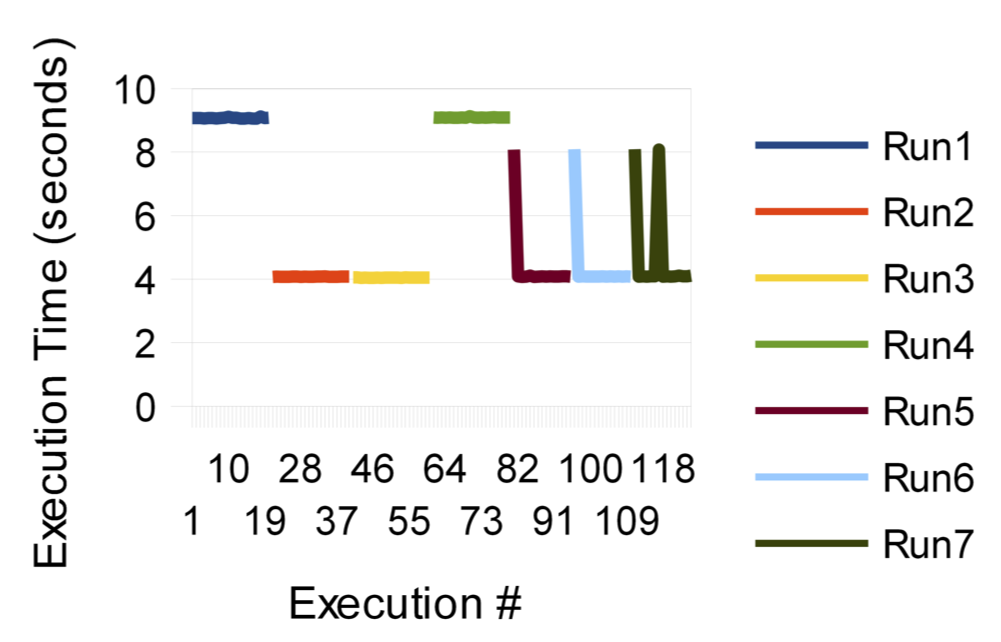
\includegraphics{_static/150_node_low_vol_object_retrieval}
\caption{Low-volume object retrival.}
\label{fig:150-node-low-vol-object-retrieval}
\end{figure}

\paragraph{Low-volume 2 -- time series}\label{low-volume-2-time-series}

\begin{lstlisting}[language=SQL]
SELECT taiMidPoint, fluxToAbMag(psfFlux), fluxToAbMag(psfFluxErr), ra, decl
FROM Source
WHERE objectId = <objId>
\end{lstlisting}

This query retrieves information from all detections of a particular
astronomical object, effectively providing a time-series of measurements
on a desired object. For testing, the objectId was randomized as for the
Low Volume 1 query, which meant that null results were retrieved where
the Source data was missing due to available space on the test cluster.

In \figref{fig:low-volume-time-series} we see that performance is roughly
constant at about 4 seconds per query. Run 1 was done after Low Volume
1's Run 1 and we discount its 9 second execution times similarly as
anomalous.

\begin{figure}[H]
\centering
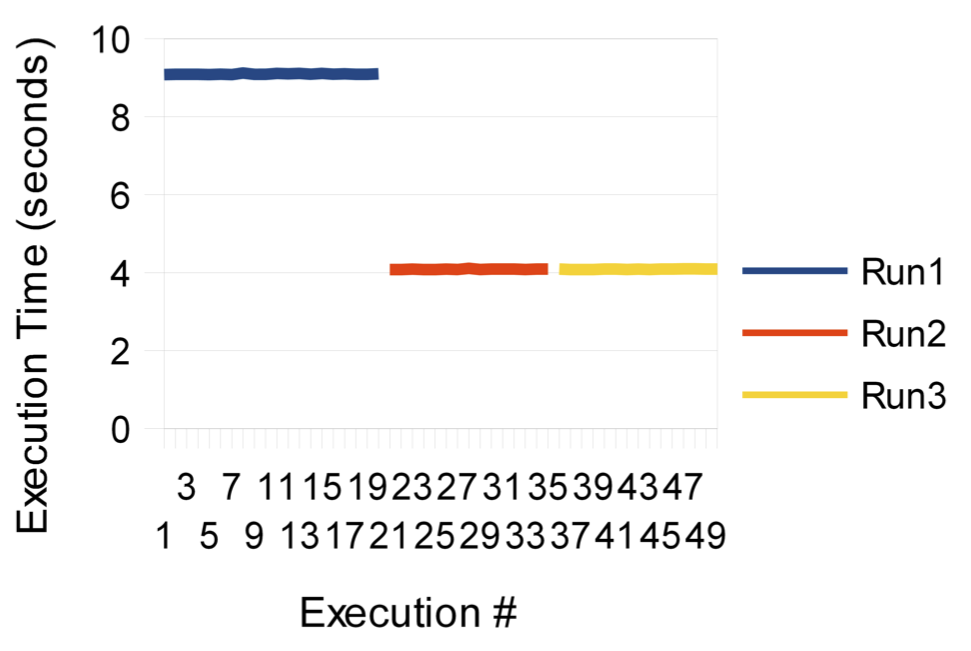
\includegraphics{_static/low_volume_time_series}
\caption{Low-volume time series.}
\label{fig:low-volume-time-series}
\end{figure}

\paragraph{Low-volume 3 -- spatially-restricted
filter}\label{low-volume-3-spatially-restricted-filter}

\begin{lstlisting}[language=SQL]
SELECT COUNT(*)
FROM Object
WHERE ra_PS BETWEEN 1 AND 2
AND decl_PS BETWEEN 3 AND 4
AND fluxToAbMag(zFlux_PS) BETWEEN 21 AND 21.5
AND fluxToAbMag(gFlux_PS)-fluxToAbMag(rFlux_PS) BETWEEN 0.3 AND 0.4
AND fluxToAbMag(iFlux_PS)-fluxToAbMag(zFlux_PS) BETWEEN 0.1 AND 0.12;
\end{lstlisting}

In \figref{fig:low-volume-spatial-filter} we see the same 4 second performance
that was seen for the other low volume queries. Again, the
\textasciitilde{}9 second performance in Run 2 could not be reproduced
so we discount it as resulting from competing processes on the cluster.

\begin{figure}[H]
\centering
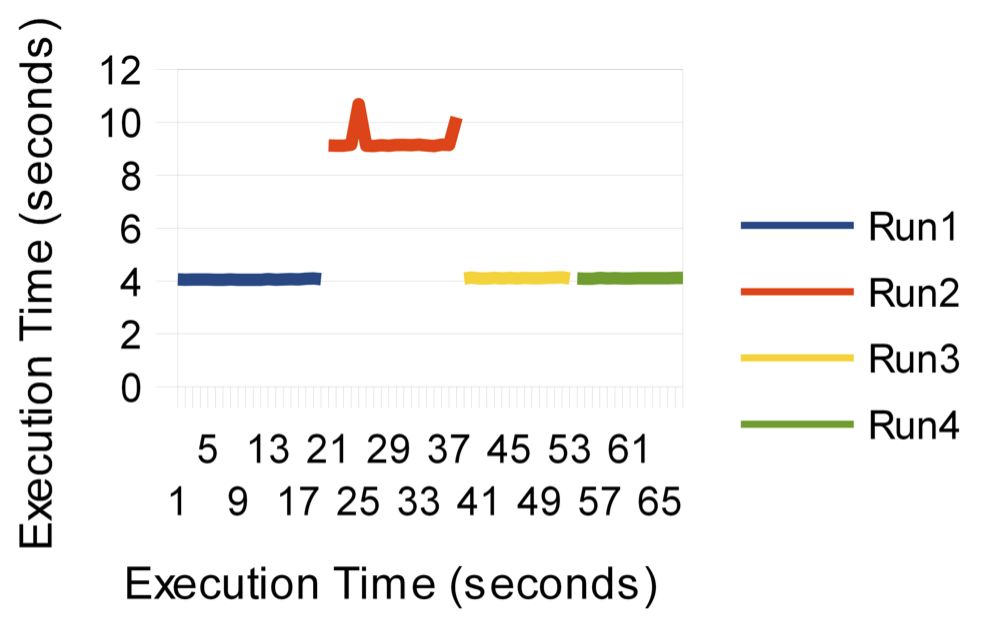
\includegraphics{_static/low_volume_spatial_filter}
\caption{Low-volume spatially-restricted filter.}
\label{fig:low-volume-spatial-filter}
\end{figure}

\paragraph{High volume 1 -- count}\label{high-volume-1-count}

\begin{lstlisting}[language=SQL]
SELECT COUNT(*) FROM Object
\end{lstlisting}

\begin{figure}[H]
\centering
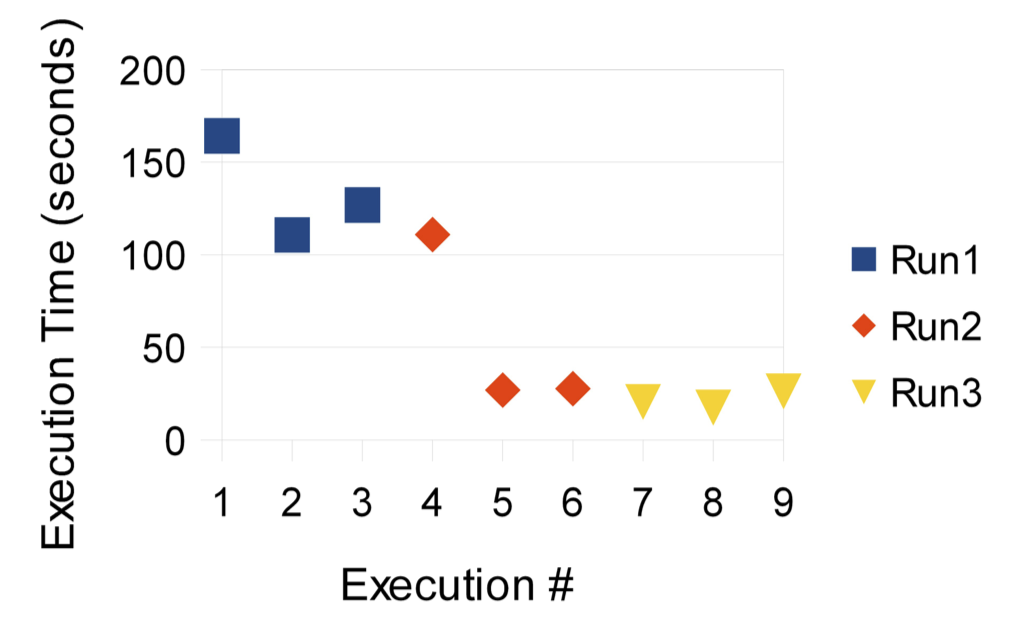
\includegraphics{_static/150_node_high_volume_count}
\caption{High volume count.}
\end{figure}

\paragraph{High-volume 2 -- full-sky
filter}\label{high-volume-2-full-sky-filter}

\begin{lstlisting}[language=SQL]
SELECT objectId, ra_PS, decl_PS, uFlux_PS, gFlux_PS,
       rFlux_PS, iFlux_PS, zFlux_PS, yFlux_PS
FROM Object
WHERE fluxToAbMag(iFlux_PS) - fluxToAbMag(zFlux_PS) > 4
\end{lstlisting}

Using the on-disk data footprint (MySQL's MyISAM .MYD, without indexes
or metadata) of the Object table (1.824x10\textsuperscript{12} bytes),
we can compute the aggregate effective table scanning bandwidth. Run 3's
7 minute execution yields 4.0GB/s in aggregate, or 27MB/s per node,
while the other runs yield approximately 11GB/s in aggregate, or 76MB/s
per node. Since each node was configured to execute up to 4 queries in
parallel, Run 3's bandwidth is more realistic, given seek activity from
competing queries and the disk manufacturer's reported theoretical
transfer rate of 98MB/s.

\begin{figure}[H]
\centering
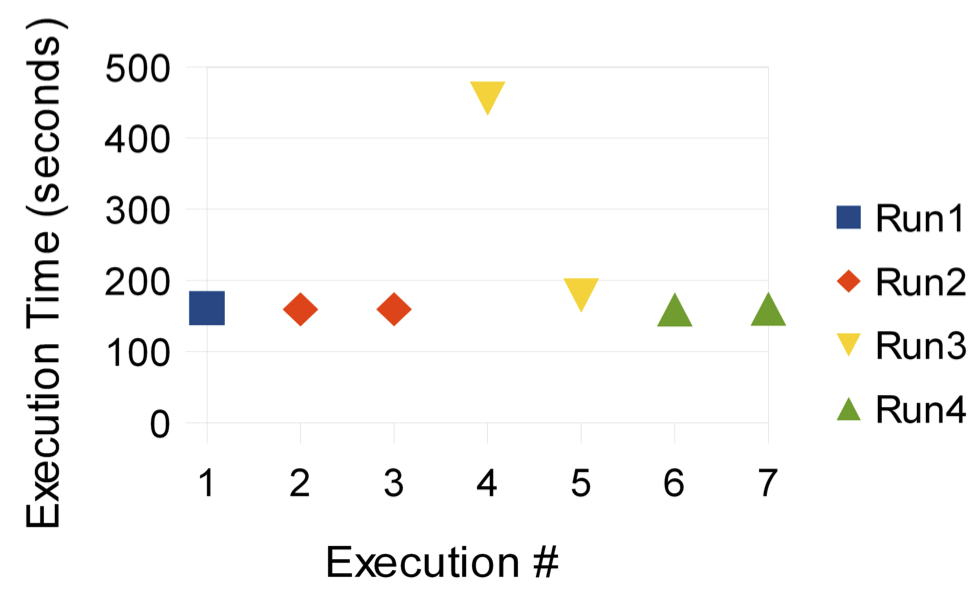
\includegraphics{_static/150_node_high_volume_full_sky}
\caption{High volume full-sky filter.}
\end{figure}

\paragraph{High-volume 3 -- density}\label{high-volume-3-density}

\begin{lstlisting}[language=SQL]
SELECT COUNT(*) AS n, AVG(ra_PS), AVG(decl_PS), chunkId
FROM Object
GROUP BY chunkId
\end{lstlisting}

\begin{figure}[H]
\centering
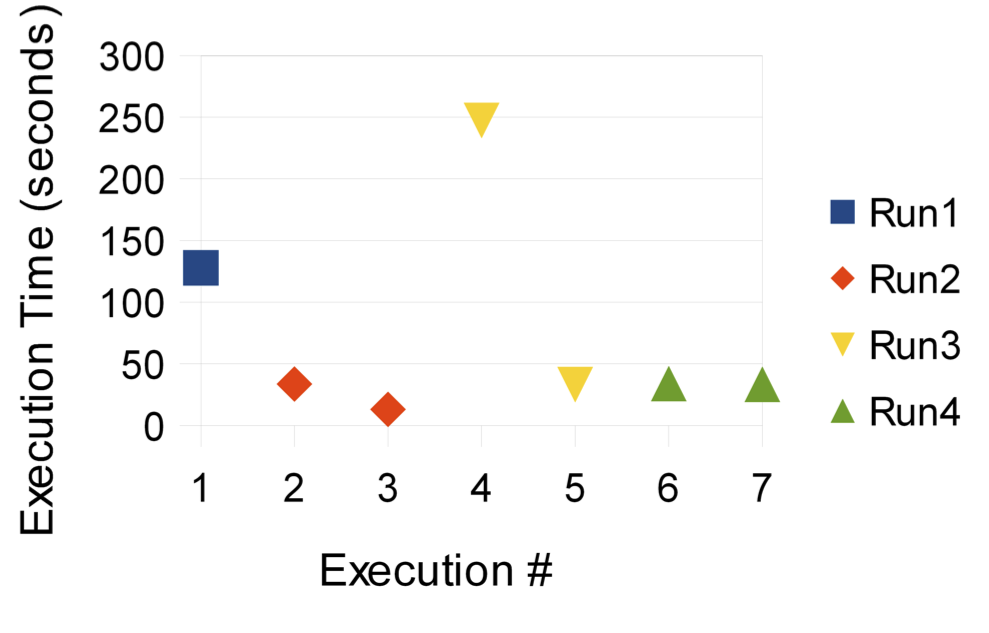
\includegraphics{_static/150_node_high_volume_density}
\caption{High volume full-sky filter.}
\label{fig:150-node-high-volume-density}
\end{figure}

This query computes statistics for table fragments (which are roughly
equal in spatial area), giving a rough estimate of object density over
the sky. It illustrates more complex aggregation query support in Qserv.
This query is of similar complexity to High Volume 2, but
\figref{fig:150-node-high-volume-density} illustrates measured times
significantly faster, which is probably due to reduced results
transmission time. As mentioned for HV2, cache behavior was not
controlled, but the 4 minute time in Run 3 may be close.

\paragraph{Super-high-volume 1 -- near
neighbor}\label{super-high-volume-1-near-neighbor}

\begin{lstlisting}[language=SQL]
SELECT COUNT(*)
FROM Object o1, Object o2
WHERE qserv_areaspec_box(-5,-5,5,-5)
AND qserv_angSep(o1.ra_PS, o1.decl_PS,
                 o2.ra_PS, o2.decl_PS) < 0.1
\end{lstlisting}

This query finds pairs of objects within a specified spherical distance
which lie within a particular part of the sky. Over two randomly
selected 100\,deg\textsuperscript{2} areas, the execution times were
about 10 minutes (667.19 seconds and 660.25 seconds). The resultant row
counts ranged between 3 to 5 billion. Since execution uses on-the-fly
generated tables, the tables do not fit in memory, and Qserv does not
yet implement caching, we expect caching effects to be negligible.

\paragraph{Super-high-volume 2 -- sources not near
objects}\label{super-high-volume-2-sources-not-near-objects}

\begin{lstlisting}[language=SQL]
SELECT o.objectId, s.sourceId, s.ra, s.decl,
       o.ra_PS, o.decl_PS
FROM Object o, Source s
WHERE qserv_areaspec_box(224.1, -7.5, 237.1, 5.5)
AND o.objectId = s.objectId
AND qserv_angSep(s.ra, s.decl, o.ra_PS, o.decl_PS) > 0.0045
\end{lstlisting}

This is an expensive query -- an \(O(kn)\) join over 150 square degrees
between a 2TB table and a 30TB table. Each objectId is unique in Object,
but is shared by 41 rows (on average) in Source, so \(k
\sim 41\). We recorded times of a few hours (5:20:38.00, 2:06:56.33, and
2:41:03.45). The variance is presumed to be caused by varying spatial
object density over the three random areas selected.

\subsubsection{Scaling}\label{scaling}

We tested Qserv's scalability by measuring its performance while varying
the number of nodes in the cluster. To simulate different cluster sizes,
the frontend was configured to only dispatch queries for partitions
belonging to the desired set of cluster nodes. This varies the overall
data size proportionally without changing the data size per node
(200-300GB). We measured performance at 40, 100, and 150 nodes to
demonstrate weak scaling.

\paragraph{Scaling with small queries}\label{scaling-with-small-queries}

From Figures \ref{fig:150-node-scaling-small-1}, \ref{fig:150-node-scaling-small-2}, and \ref{fig:150-node-scaling-small-3}, we
see that execution time is unaffected by node count given that the data
per node is constant. The spike in the 40-node configuration in
\ref{fig:150-node-scaling-small-3} is caused by 2 slow queries (23s and 57s);
the other 28 executed in times ranging from 4.09 to 4.11 seconds.

\begin{figure}[H]
\centering
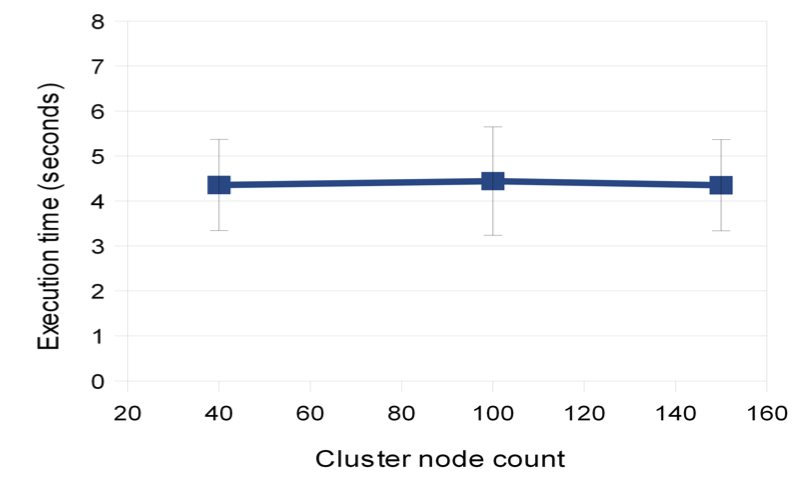
\includegraphics{_static/150_node_scaling_small_1}
\caption{Scaling with node count (1).}
\label{fig:150-node-scaling-small-1}
\end{figure}

\begin{figure}[H]
\centering
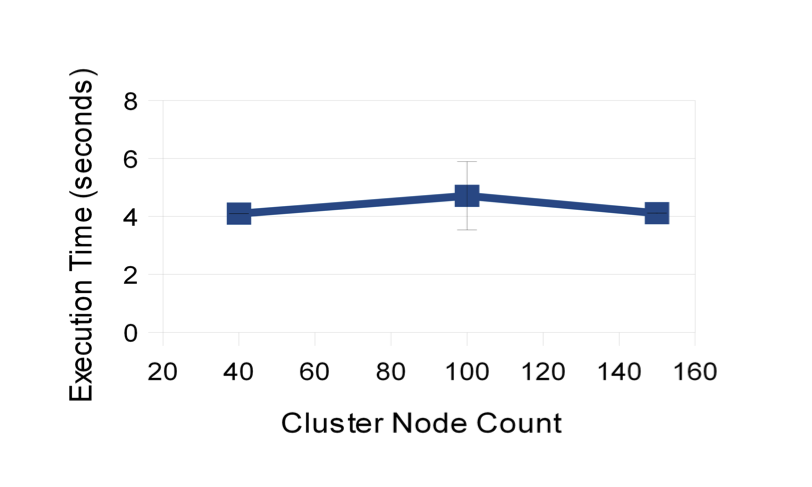
\includegraphics{_static/150_node_scaling_small_2}
\caption{Scaling with node count (2).}
\label{fig:150-node-scaling-small-2}
\end{figure}

\begin{figure}[H]
\centering
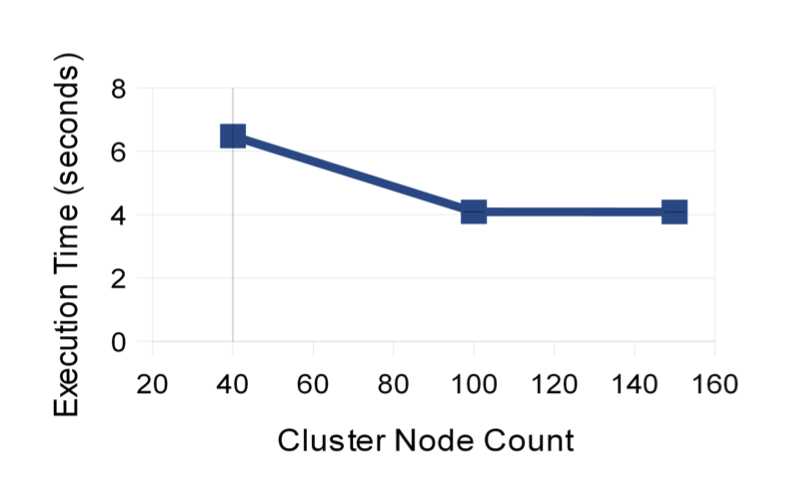
\includegraphics{_static/150_node_scaling_small_3}
\caption{Scaling with node count (3).}
\label{fig:150-node-scaling-small-3}
\end{figure}

\paragraph{Scaling with expensive
queries}\label{scaling-with-expensive-queries}

\textbf{High Volume}

If Qserv scaled perfectly linearly, the execution time should be
constant when the data per node is constant. In
\figref{fig:150-node-scaling-high-volume} the times for high volume queries show
a slight increase. HV1 is a primarily a test of dispatch and result
collection overhead and its time increases linearly with the number of
chunks since the front-end has a fixed amount of work to do per chunk.
Since we varied the set of chunks in order to vary the cluster size, the
execution time of HV1 should thus vary linearly with cluster size. HV3
seems to have a similar trend since due to cache effects -- its result
was cached so execution became more dominated by overhead.

The High Volume 2 query approximately exhibits the flat behavior that
would indicate perfect scalability. Caching effects may have clouded the
results, but they did not dominate. If the query results were perfectly
cached, we expect the overall execution time to be dominated by overhead
as in HV1, and this is clearly not the case.

\begin{figure}[H]
\centering
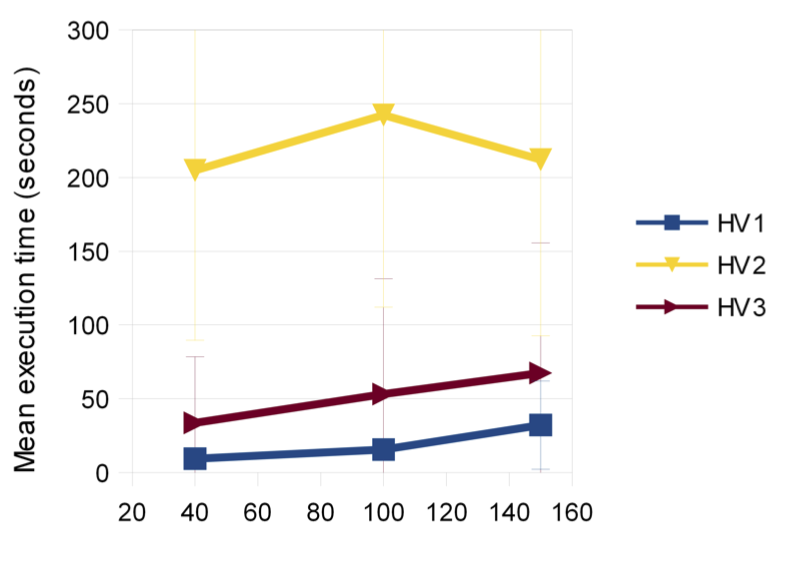
\includegraphics{_static/150_node_scaling_high_volume}
\caption{Scaling with high volume queries.}
\label{fig:150-node-scaling-high-volume}
\end{figure}

\textbf{Super High Volume}

The tests on expensive queries did not show perfect scalability, but
nevertheless, the measurements did show some amount of parallelism. It
is unclear why execution in the 100-node configuration was the slowest
for both SHV1 and SHV2. Our time-limited access to the cluster did not
allow us to repeat executions of these expensive queries and study their
performance in better detail.

\begin{figure}[H]
\centering
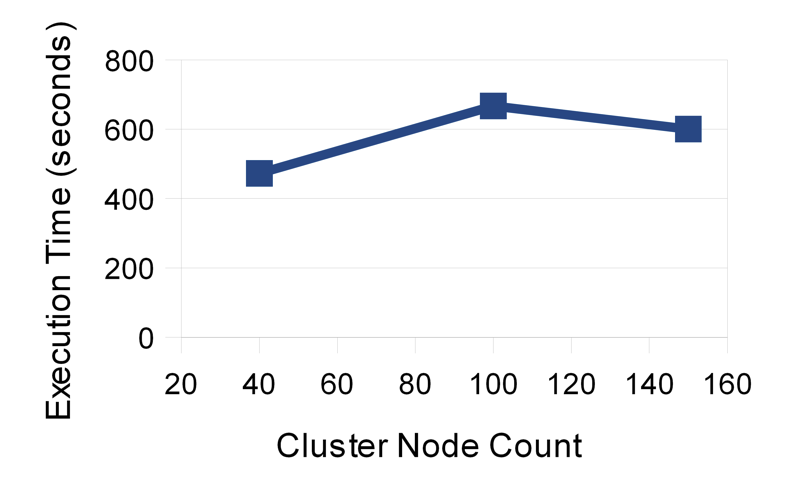
\includegraphics{_static/150_node_super_high_volume}
\caption{Scaling with super high volume queries.}
\end{figure}

\subsubsection{Concurrency}\label{concurrency}

\begin{figure}[H]
\centering
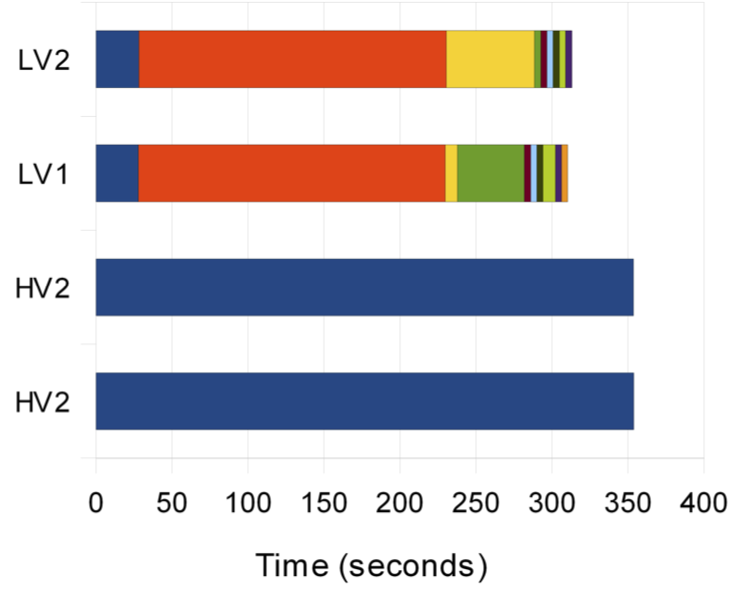
\includegraphics{_static/150_node_concurrency}
\caption{Concurrency test.}
\end{figure}

We were able to test Qserv with multiple queries in flight. We ran 4
``streams'' of queries: two parallel invocations of HV2, one of LV1, and
one of LV2. Each low volume stream paused for 1 second between queries.
Figure 12 illustrates concurrent performance. We see that the HV2
queries take about twice the time (5:53.75 and 5:53.71) as they would if
running alone. This makes sense since each is a full table scan that is
competing for resources and shared scanning has not been implemented.
The first queries in the low volume streams execute in about 30 seconds,
but each of their second queries seems to get ``stuck'' in queues. Later
queries in the streams finish faster. Since the worker nodes maintain
first- in-first-out queues for queries and do not implement any concept
of query cost, long queries can easily hog the system. The slowness of
low volume queries after the second queries may be curious at first
glance, since they should be queued at the end on their assigned worker
nodes and thus complete near the end of the HV2 queries. In that case,
subsequent queries would land on workers with nearly empty queues and
execute immediately. This slowness can be explained by query skew --
short queries may land on workers that have or have not finished their
work on the high volume queries.

\subsubsection{Discussion}\label{discussion-1}

\paragraph{Latency}\label{latency}

LSST's data access needs include supporting both small, frequent,
interactive queries and longer, hour/day-scale queries. We designed
Qserv to operate efficiently in both cases to avoid needing multiple
systems, which would be costly in development, maintenance, and
hardware. Indexing was implemented in order to reduce latency for cheap
queries that only touch a small part of the data.

The current Qserv implementation incurs significant overhead in
dispatching queries and collecting results. In early development we
decided to minimize the intelligence on each worker, so the front-end
master became responsible for preparing the SQL queries so that workers
did not need to perform parsing or variable substitution. Results
collection is somewhat heavyweight as well. MySQL does not provide a
method to transfer tables between server instances, so tables are dumped
to SQL statements using \emph{mysqldump} and reloaded on the front-end.
This method was chosen to speed prototyping, but its costs in speed,
disk, network, and database transactions are strong motivations to
explore a more efficient method.

\paragraph{Solid-state storage}\label{solid-state-storage}

Some of Qserv's design choices (e.g., shared scanning) are motivated by
the need to work around poor seek performance characteristics of disks.
Solid-state storage has now become a practical alternative to mechanical
disk in many applications. While it may be useful for indexes, its
current cost differential per unit capacity means that it is still
impractical to store bulk data. In the case of flash storage, the most
popular solid-state storage technology, shared scanning is still
effective in optimizing performance since DRAM is much faster than flash
storage and flash still has ``seek'' penalty characteristics (though it
is much better than spinning disk).

\paragraph{Many core}\label{many-core}

We expect the performance to be I/O constrained, since the workload is
data, not CPU performance limited. It is unlikely that many cores can be
leveraged on a single node since they will be sized with only the number
of disk spindles that saturate the north bridge, but shared scanning
should increase CPU utilization efficiency.

\paragraph{Alternate partitioning}\label{alternate-partitioning}

The rectangular fragmentation in right ascension and declination, while
convenient to visualize physically for humans, is problematic due to
severe distortion near the poles. We are exploring the use of a
hierarchical scheme, such as the hierarchical triangular mesh
\citep{2001misk.conf..631K} for partitioning and spatial indexing. These schemes can
produce partitions with less variation in area, and map spherical points
to integer identifiers encoding the points' partitions at many
subdivision levels. Interactive queries with very small spatial extent
can then be rewritten to operate over a small set of fine partition IDs.
If chunks are stored in partition ID order, this may allow I/O to occur
at below sub-chunk granularity without incurring excessive seeks.
Another bonus is that mature, well tested, and high-performance open
source libraries exist for computing the partition IDs of points and
mapping spherical regions to partition ID sets.

\paragraph{Distributed management}\label{distributed-management}

The Qserv system is implemented as a single master with many workers.
This approach is reasonable and has performed adequately in testing, but
the bottlenecks are clear. A Qserv instance at LSST's planned scale may
have a million fragment queries in flight, and while we have plans to
optimize the query management code path, managing millions from a single
point is likely to be problematic. The test data set described in this
paper is partitioned into about 9,000 chunks, which means that a launch
of even the most trivial full-sky query launches about 9,000 chunk
queries.

One way to distribute the management load is to launch multiple master
instances. This is simple and requires no code changes other than some
logic in the MySQL Proxy to load-balance between different Qserv
masters. Another way is to implement tree-based query management.
Instead of managing individual chunk queries, the master would dispatch
groups of them to lower-level masters which would could either subdivide
and dispatch subgroups or manage the individual chunk queries
themselves.

\subsection{100-TB Scalability Test (JHU 20-node
cluster)}\label{tb-scalability-test-jhu-20-node-cluster}

In the fall of 2012, we were provided the opportunity to use a cluster
of computers at John Hopkins University (JHU), that were large memory,
multi-processor computers, each with very large storage attached, to
setup as a Qserv service. There were 21 nodes provided for us, and the
nodes had two processors with 12 cores each of Intel Xeon X5650 CPUs at
2.67GHz. But mounted as a data volume, were 22TB raid arrays, to provide
a possible 450TB of storage. This would provide a high volume storage
test, but with a low number of compute nodes, with one master node, and
20 worker nodes.

The data used would be produced on each node, starting with a test
dataset called ``pt12''. This test dataset was 220GB, but high density
data in one particular spot in the sky, a few degrees wide. We chose a
high density spot of this data, and then duplicated with across the
whole sphere, to provide a high density dataset over the whole sky,
yielding an estimated 100TB of data.

The production of this large amount of data proved to have problems. The
production was rather slow, taking many weeks for a full production on
each node. At first long processes were setup, and the stability of the
cluster was an issue, with processes dying after days of running, and
many smaller production processes were setup to get past stability
issues. This produced over 100TB of csv text files, into about 7000
chunks worth of data. Once that was done, then this data was loaded into
MySQL MyISAM tables, and with the large data sizes this also took days.

Over the course of this time, often nodes would go out with problems,
and be down for some amount of time, before coming back. Often this
would be with the data still on the mounted volumes, but the loss of
computing nodes would set back the time until the data would be
complete. But this was a small problem, than the problem of data
stability. Once all the nodes were up and running, the data service was
still having problems. This was found to be either loss or corruption of
a few of the thousands of tables on the various nodes. With loss of
data, either data would be re-created or just blocked for testing. Over
the course of testing, dealing with data corruption was constant issue,
but still a large percentage would be accessible at least. Also a
problem was file corruption on the install software, and a few nodes
needed to be reinstalled over the course of the testing. A full 100TB of
data was generated, but only about 85TB could ever be served, before the
resources had to be given back.

But some testing was able to get done on this cluster. A full table scan
was performed on the Object data, although this was only on the aprox,
85TB of data was served, not the complete 100TB of data that was
generated. The query was performed:

\begin{lstlisting}[language=SQL]
SELECT count(*) FROM Object
\end{lstlisting}

\begin{verbatim}
+------------+
| count(*)   |
+------------+
| 2059335968 |
+------------+

1 row in set (19.26 sec)
\end{verbatim}

Showing 2B objects in the table. The result here was after the query was
performed a few times, and the cache had been stabilized. This is
similar to the times found from previous testing.

The low volume test from access to a small portion of the sky was also
performed. Using the query:

\begin{lstlisting}[language=SQL]
SELECT count(*)
FROM Object
WHERE qserv_areaspec_box(1,3,2,4)
AND scisql_fluxToAbMag(zFlux_PS) BETWEEN 21 AND 21.5
\end{lstlisting}

\begin{verbatim}
+----------+
| count(*) |
+----------+
| 748      |
+----------+

1 row in set (4.45 sec)
\end{verbatim}

This time for access is also similar to previous testing, looking for
the number of object in a small part of the sky of a certain color. The
\textasciitilde{}4.5 sec. overhead here is a baseline overhead for data
access in this version of the qserv software.

A high volume data test was performed, looking for color information on
records within a certain range of color. This will scan over all
objects, to return certain number of records. The test query was:

\begin{lstlisting}[language=SQL]
SELECT objectId, ra_PS, decl_PS, uFlux_PS, gFlux_PS,
       rFlux_PS,iFlux_PS, zFlux_PS, yFlux_PS
FROM Object
WHERE scisql_fluxToAbMag(iFlux_PS) -
      scisql_fluxToAbMag(zFlux_PS) > 4
\end{lstlisting}

This query returned 15695 records in 6 min 33.50 sec. Again this query
was performed a number of times, and this time is the average time after
the caches had stabilized. This query was performed again, this time
looking at a lower number of records, looking for the difference between
\emph{i} and \emph{z} flux of 5 this time. This query returned 2967
records, in 6 min 14.0 sec. The time was a little lower this time, which
was mostly the time to print the records to the screen, where the rest
of the time was the over-head in scanning the available object data to
return these records. The previous tests were done on 30TB of data, but
using 150 nodes, although these nodes had many less cores. But this test
would return in about 180 sec there, where here it is about 375 sec. The
extra time here will come from the access of larger amounts of data per
node, and amount of data in general, and the access rate of the data
storage.

\subsection{Concurrency Tests (SLAC 100,000
chunk-queries)}\label{concurrency-tests-slac-100000-chunk-queries}

A previous version of the Qserv master code had dedicated two fixed size
thread pools to each query, one for dispatching chunk queries, and the
other for reading back results. The dispatch pool was sized at a quite
high 500 threads for two reasons. Firstly, one goal was to dispatch work
as quickly as possible, allowing the Qserv workers to prioritize as they
know best. Secondly, the first query dispatch against a chunk takes
\textasciitilde{}5\,s, so that cluster cold start latency on a full table
scan of \textasciitilde{}10,000 chunks takes approximately 100\,s with
this many dispatch threads. Subsequently,
XRootD caching allows for near instantaneous
dispatches in comparison.

The thread pool for result reads was given a much smaller size: just 20
threads per query. This is because the Qserv master process can only
exploit limited amounts of parallelism when merging worker results for a
single query. In fact, the main benefit of using a number as high as 20
threads is that it reduces result merge latency when chunk query
execution times (and hence result availability times) are skewed.

An unfortunate consequence of this simple design was that running too
many concurrent queries would cause thread creation failures in the
Qserv master process. We therefore changed to a unified query dispatch
and result reader thread pool model.

To test our ability to handle many concurrent full-table scan queries
without running out of threads, we partitioned the PT1.2 Object table
into \textasciitilde{}8,000 chunks, and distributed them across an 80
node cluster at SLAC. The nodes in this cluster were quite old and had
limited quantities of RAM, making them the perfect workhorses for this
sort of test. In particular, asking for more than \textasciitilde{}1000
threads would cause Qserv master failure on this platform. Using the new
unified thread-pool design we were able to successfully run between 2
and 12 concurrent Object table scans each involving
\textasciitilde{}8,000 chunk queries, requiring a total execution time
of 2 to 8 minutes, thus demonstrating that the Qserv master can handle
loads of \textasciitilde{}100,000 in-flight chunk queries, even on very
old hardware.

Note that using a unified thread pool for result reads requires special
measures to avoid query starvation. A single query can easily require
10,000 result reads and there will be far fewer total threads in the
pool. As a result, we must be careful to avoid assigning all threads to
a single query, or queries that should be interactive can easily become
decidedly non-interactive as they wait for a table scan to finish. Our
unified thread pool implementation therefore assigns available threads
to the query using the fewest worker threads, and makes sure to create
new threads when a new query is encountered (up to some hard limit).

To test this, we setup Qserv with a single master node and a single
worker node. The worker was configured with \textasciitilde{}12,000
empty chunk tables. We then submitted both full-table scans
(\texttt{SELECT\ COUNT(*)\ FROM\ Object}), and an interactive query
(\texttt{SELECT\ COUNT(*)\ FROM\ Object\ WHERE\ objectId\ IN\ (1)})
requiring just a single chunk query to answer. Though we were able to
demonstrate that the master immediately allocated threads to dispatch
the lone interactive chunk query and read back its results, the
execution time of the interactive query was still far higher than it
should have been. It turns out this is because the Qserv worker uses a
FIFO chunk query scheduling policy, and the single chunk query
corresponding to the interactive user query was being queued up behind a
multitude of chunk queries from the full table scan on the worker side.
We are currently working to address this deficiency as part of ongoing
work on shared scans.

\bibliography{lsst,lsst-dm,refs_ads}

\end{document}
